\section{Economics of SDP}\label{sec:econ}

% The main goal of smart data pricing is to relieve network congestion by incentivizing users to alter their behavior. Using pricing as an incentive mechanism is not a new idea--indeed, it might be said that most pricing plans exist to incentivize users! Regarding mobile data usage specifically, one can divide the prior literature into two categories: \emph{static pricing}, in which the offered prices are essentially fixed and change on a timescale of months or years, and \emph{dynamic pricing}, in which the prices offered change on a timescale of seconds or hours. In this chapter, we use one example of static and one example of dynamic pricing to elucidate key economic concepts useful for smart data pricing research.

Given the wide variety of SDP pricing algorithms presented in Section \ref{sec:congestion}, a thorough discussion of the theory behind each one is impractical for a book chapter. In this section, we instead select four representative scenarios to illustrate some of the key economic principles often used in formulating different types of pricing algorithms. We first consider static pricing on a single link, and then consider both real-time dynamic pricing and day-ahead time-dependent pricing. Readers familiar with network economics may wish to skip this section.

\subsection{Usage-Based Pricing: A Single Link Example}\label{sec:single}

An operator generally sets its mobile data prices so as to achieve a certain objective, e.g., maximizing profit. In this section, we review some standard economic concepts that are often used in formulating such objective functions. We consider two agents: end users and ISPs.\footnote{Sponsored content and app-based pricing models may also include content providers as a separate type of agent.} For simplicity, we consider only one ISP with a given set of customers, and we suppose that the ISP wishes to build a last-mile access link in its network. The ISP wishes to determine both the \emph{capacity to provision} on this link, as well as the \emph{price per unit bandwidth} to charge its users on the link. This is a standard monopolist profit maximization that we discuss below. We denote the capacity with the variable $x$, and the price by the variable $p$. The ISP-user interaction is summarized in Figure \ref{fig:supply-demand}.

\begin{figure}
\centering
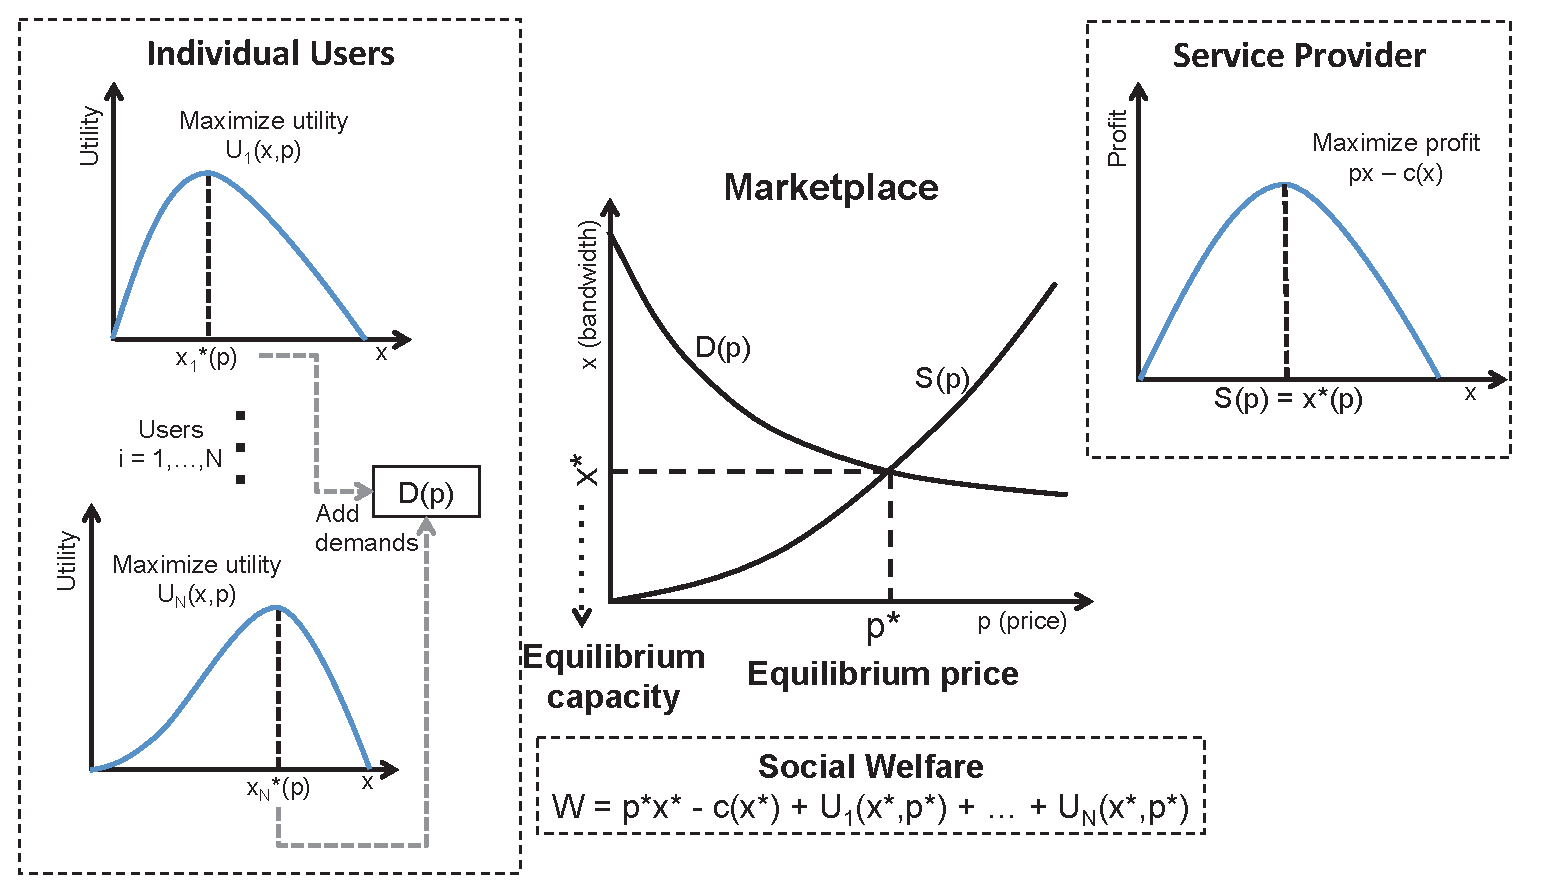
\includegraphics[width = 0.8\textwidth]{Figures/Supply_Demand.eps}
\caption{User-ISP interaction in a mobile data marketplace.}
\label{fig:supply-demand}
\end{figure}

We first consider users' decisions to purchase certain amounts of bandwidth on the ISP's new access link. In modeling this user behavior, we suppose that each user acts so as to maximize his or her \emph{consumer surplus function}, denoted by $U_j(x_j,p)$ for each customer $j = 1,2,\ldots, J$. The function $U_j$ is the net benefit to a consumer from the utility received in purchasing $x_j$ amount of bandwidth for a price $p$ per unit bandwidth.\footnote{This function may be additively decomposed into the form $U_j(x_j,p) = V_j(x_j) - px_j$, i.e., a utility term $V_j$ and the price paid $px_j$. In this scenario, $V_j(x_j)$ is often called the utility, and $U_j(x_j,p)$ the net benefit received by the user. Additively incorporating the price can also be interpreted as incorporating user budget constraints through Lagrange multipliers; more details can be found in Section \ref{sec:realtime}.} Thus, given a price $p$, if $U_j(y_j, p) > U_j(x_j,p)$, user $j$ prefers to purchase $y_j$ units of bandwidth, rather than $x_j$ units. Since the ISP chooses the value of $p$, each user $j$ takes the price as given and chooses the quantity of bandwidth to purchase $\left(x_j\right)$ so as to maximize the utility $U_j(x_j, p)$. We denote this utility-maximizing quantity as $x_j^\ast(p)$.\footnote{The argument $p$ emphasizes the fact that this optimal bandwidth $x_j^\ast$ depends on the price $p$ offered by the ISP.} These functions $x_j^\ast(p)$ are called users' \emph{demand functions}; adding them up, we obtain the \emph{aggregate demand function}, $D(p) = \sum_j x_j^\ast(p)$.

We now consider the ISP's problem of choosing a link capacity $x$ and price $p$. Given a price $p$ and assuming full utilization of the link capacity, the ISP chooses $x$ so as to maximize its utility function. Usually, the ISP's utility is simply its \emph{profit}, but other functions can be used. We write the ISP profit as $px - c(x)$, where $px$ is the ISP revenue and the function $c(x)$ denotes the cost of building a link of capacity $x$. Given $p$, the ISP can then find $x^\ast(p)$, the optimal link capacity as a function of the price $p$. We use $S(p) = x^\ast(p)$ to denote this supply side function.

When the user and ISP are at a \emph{market equilibrium}, supply equals demand: $D(p) = S(p)$. At such a price $p^\ast$ satisfying this relation, each user maximizes his or her own utility by purchasing $x_j^\ast\left(p^\ast\right)$ amount of bandwidth, and the ISP maximizes its utility by providing just enough capacity $x^\ast\left(p^\ast\right) = \sum_j x_j^\ast\left(p^\ast\right)$ to support those users' demands.
%
One often-analyzed property of this equilibrium is the \emph{social welfare}, defined as the sum of the utility received by all users $j$ and the ISP:
\begin{equation*}
\sum_j U_j\left(x_j^\ast,p^\ast\right) + p^\ast\sum_j x_j^\ast\ - c\left(\sum_j x_j^\ast\right),
\end{equation*}
where $x_j^\ast$ is understood to be evaluated at the equilibrium price $p^\ast$. This social welfare can be divided into two portions: the \emph{user surplus}, or the sum of user utilities, and the \emph{ISP surplus}, or the utility (here, profit) obtained by the ISP. Depending on the utility functions $U_j$ and the cost function $c$, the total social welfare may change, and the users and ISP may receive different portions of the overall social welfare.

Before moving on, we pause to discuss some of the more common extensions of the simple problem above. One is to introduce \emph{budget constraints} on each user's utility maximization problem: the user may not want to spend more than a certain amount $B_j$, in which case each user $j$ maximizes the utility $U_j(x_j,p)$ subject to the constraint $px_j \leq B_j$. We may also consider a situation in which users impose \emph{externalities} on each other, i.e., a given user $j$'s utility is affected by the capacity allocated to other users $i\neq j$. For instance, there may be a positive externality in which user $j$'s utility increases as other users send traffic over the link in order to interact with user $j$. On the other hand, one could also observe negative externalities, in which congestion from other users' traffic diminishes a particular user's utility, e.g., by increasing delay.

When solving for the market equilibrium above, we initially took the price $p$ as fixed for the end users and ISP, and then found the equilibrium market price $p^\ast$. In fact, one can obtain this equilibrium price by only examining the optimal behavior of end users and ISPs, i.e., without explicitly considering market equilibrium. Suppose that the ISP, knowing users' demand functions $x_j^\ast(p)$, calculates its revenue as a function of price to be $p\sum x_j^\ast(p)$ (the price, multiplied by the user demand as a function of price). The ISP can then choose both $p$ and $x$ so as to maximize its profit $p\sum_j x_j^\ast(p) - c(x)$, subject to the constraint that the link capacity be able to accommodate users' total demand $\sum_j x_j^\ast$, i.e., that $x \geq \sum_j x_j^\ast$. It is easy to see that (assuming the cost $c(x)$ is increasing in the capacity $x$), at the optimum, $x = \sum_j x_j^\ast$. The ISP then chooses the optimal price $p$ so as to maximize $p\sum_j x_j^\ast(p) - c\left(\sum_j x_j^\ast(p)\right)$. One can show that the resulting optimal price, which we will call $\overline{p}$, is the same equilibrium price $p^\ast$ obtained above: at $\overline{p}$, each user $j$ demands $x_j^\ast(\overline{p})$, and the ISP chooses its optimal capacity $x^\ast(\overline{p})$. This is exactly the point at which the supply and demand curves intersect, i.e., $p^\ast$.

The above reasoning, in which an ISP chooses a price to offer subject to users' behavior as a function of the price chosen, is a simple example of a \emph{game} between users and ISPs. In such a game, several players interact with each other, and each player acts to maximize his or her own utility, which may be influenced by other players' decisions. For instance, in this scenario, users interact with the ISP by utilizing the access link in its network and paying some price. Their decisions on how much capacity to utilize (i.e., choosing $x_j^\ast$) are influenced by the ISP's choice of the price $p$. This interpretation of the single-link example leads us to next consider some basic principles of \emph{game theory} in relation to SDP.

\subsection{Incentive Compatibility: Game-Theoretic Principles}\label{sec:gametheory}

To illustrate some of the basics of game theory, we again consider the single link example above. The user-ISP interaction in such a scenario is an example of a \emph{Stackelberg game}, in which one player, the ``leader,'' makes a decision (e.g., the ISP sets a unit price $p$ for link capacity) and the remaining players, or ``followers,'' then make their own decisions based on the leader's actions. In SDP, this framework reflects the need to consider users' and ISPs' optimal actions when choosing pricing policies that incentivize particular types of resource allocations. In this example, users choose their demands $x_j^\ast(p)$, given the ISP's price $p$. Stackelberg games, which often arise in user-ISP interactions, may be solved using \emph{backwards induction}: first, one computes the followers' actions as a function of the leader's decision (in our example, we compute the functions $x_j^\ast(p)$). The followers' actions are sometimes called a \emph{best response} to the leader. The leader then takes these actions into account and makes his or her own decision (given that users' demands are $x_j^\ast(p)$, the ISP chooses the optimal price $p$). This decision is then the best response to the followers.

The backwards induction process leads to a \emph{subgame perfect equilibrium} in the Stackelberg game: at this equilibrium, each player is maximizing his or her own utility, and no player has an incentive to change his or her behavior. To formalize this definition, we will need to first explain the concept of a \emph{Nash equilibrium}. Consider a general game with $n$ users, each of whom can take an action, e.g., by choosing the value of a variable $y_j$; $j = 1,2,\ldots,n$; and suppose that each user $j$'s utility $V_j$ is a function of all of the $y_j$ variables, i.e., $V_j = V_j\left(y_1,y_2,\ldots,y_n\right)$. Then a set of actions $z_1,\ldots,z_n$ is a Nash equilibrium if $V_j\left(z_1,\ldots,z_j,\ldots,z_n\right) \geq V_j\left(z_1,\ldots,y_j,\ldots,z_n\right)$ for any $y_j \neq z_j$. In other words, assuming that all the other players take actions $z_i$, player $j$'s action $z_j$ optimizes its utility $V_j$.

We may generalize the concept of a Nash equilibrium to a Stackelberg game's subgame-perfect equilibrium by considering \emph{subgames} of the Stackelberg game. We do not give the general definition of a subgame here, but it may be understood by envisioning the Stackelberg game as a dynamic game with different levels defined by the time of decision: on the first level, users make their decisions, and on the second, ISPs make their decisions. A subgame encompasses a group of players who mutually interact, but do not directly interact with other players at their level. In our scenario, a subgame would be a subset of users and the ISP. A subgame-perfect equilibrium of the full Stackelberg game is then a set of actions that comprise a Nash equilibrium in each subgame of the full game. It can be shown that any equilibrium found from backwards induction is a subgame-perfect equilibrium; one can easily check that this is the case in our example scenario. Nash and subgame-perfect equilibria are considered stable in that once they have been achieved, no user has an incentive to change their behavior. (Unfortunately, one cannot in general guarantee that such an equilibrium will be achieved in the first place, and a game may have multiple Nash equilibria.)

Another type of game that often arises in SDP is that of competing service providers. For instance, we may have an \emph{oligopoly} of a few companies who dominate the market for mobile data, e.g., AT\&T and Verizon in the United States are the dominant market players. Each of these companies then competes for customers (i.e., market share) and revenue with the others. This competition defines their interactions, and each company can try to make strategic decisions that optimize its market share. Given a mathematical model of the companies' actions, one can then try to study the corresponding game, e.g., by computing possible Nash equilibria.

While certainly useful for explicit pricing problems like that considered above, game theory can also be applied to more general resource allocation problems, just as SDP allows ISPs to incentivize users to consume data so as to realize particular resource allocations. To illustrate these uses, we again consider the single link example, but we now suppose that the link's capacity is fixed and that the ISP wishes to allocate this fixed amount of capacity $x$ among its $n$ users.

If users selfishly maximize their individual utilities (i.e., choose demands $x_j^\ast(p)$), then the ISP can set a virtual price $p$ to force an allocation in which $\sum_j x_j^\ast(p) = x$, i.e., all of the available capacity is utilized, and each user maximizes his or her utility. This price serves as a signal through which the ISP can control users' demands. However, such an allocation may be unfair: very price-sensitive users may be able to afford significantly less capacity than others. Since revenue is no longer involved, the ISP can afford to care about other objectives like fairness. Indeed, a vast literature exists on just such a problem; we will not go into fairness theory here, but we will present one approach inspired by game theory.

In the Stackelberg game discussed above, users did not cooperate: each user maximized only his or her own utility, subject to the ISP's offered price. Yet if users do cooperate, they may reach a better decision. We can study this problem by first defining individual users' utilities $U_j(y_j)$; given a capacity amount $y_j$, each user $j$ derives utility $U_j(y_j)$. For instance, users could jointly choose their demands $y_j$, subject to the capacity constraint $\sum_j y_j \leq x$, so as to maximize an overall utility function $U\left(U_1(y_1),\ldots,U_n(y_n)\right)$. Depending on the choice of $U$, of course, one would obtain different allocations $y_j^\ast$. We use $y_j^\ast$ to denote the $y_j$ that jointly maximize $U$. Nash proposed that the $y_j^\ast$ satisfy the following four axioms:
\begin{enumerate}
\item
\emph{Invariant to affine transformations:} For each user $j$, define the utility function $V_j(y_j) = \alpha_j U_j(y_j) + \beta_j$ for some constants $\alpha_j > 0$, $\beta_j$. Then the allocation $\left\{z_j^\ast\right\}$ maximizing $U\left(V_1(z_1),\ldots,V_n(z_j)\right)$ satisfies $V_j\left(z_j^\ast\right) = \alpha_jU_j\left(y_j^\ast\right) + \beta_j$ for each user $j$, where the allocation $\left\{y_j^\ast\right\}$ maximizes $U\left(U_1(y_1),\ldots,U_n(y_n)\right)$. An affine transformation of the utility functions $U_j$ does not change the utility received at the optimal allocation.
\item
\emph{Pareto-optimality:} An allocation $\left\{y_1^\ast,\ldots,y_n^\ast\right\}$ is Pareto-optimal if for any user $j$, any feasible allocation $\left\{z_1,\ldots,z_n\right\}$ with $U_j(z_j) > U_j\left(y_j^\ast\right)$ satisfies $U_i(z_i) < U_i\left(y_i^\ast\right)$ for some user $i$. In other words, no user can be made better off without making another worse off.
\item
\emph{Independence of irrelevant alternatives:} Suppose that $U\left(U_1(y_1),\ldots,U_n(y_n)\right) > U\left(U_1(z_1),\ldots,U_n(z_n)\right)$ for two feasible allocations $\left\{y_j\right\}$ and $\left\{z_j\right\}$. Then if the problem constraints are relaxed to allow new feasible allocations, we still have $U\left(U_1(y_1),\ldots,U_n(y_n)\right) > U\left(U_1(z_1),\ldots,U_n(z_n)\right)$.
\item
\emph{Symmetry:} Suppose that $\left\{y_1,\ldots,y_n\right\}$ and $\left\{z_1,\ldots,z_n\right\}$ are feasible capacity allocations with $U_{j_1}(y_{j_1}) = U_{j_2}(z_{j_2})$ for some users $j_1$ and $j_2$, $U_{j_2}(y_{j_2}) = U_{j_1}(z_{j_1})$, and $U_j(y_j) = U_j(z_j)$ for all $j\neq j_1, j_2$. Then $U\left(U_1(y_1),\ldots,U_n(y_n)\right) = U\left(U_1(z_1),\ldots,U_n(z_n)\right)$. In other words, switching the order of the utilities received does not change the overall utility $U$.
\end{enumerate}
An allocation satisfying these four axioms is said to be a \emph{Nash bargaining solution}. One can show that if $U$ is taken to be $\prod_j U_j(y_j)$, then the resulting $y_j^\ast$ is a Nash bargaining solution. Taking the logarithm, we see that this is equivalent to maximizing $\sum_j \log\left(U_j(y_j)\right)$. In other words, users choose their demands to maximize the sum of the \emph{logarithms} of their utilities $U_j$. Since the logarithm is sub-linear for large $U_j(y_j)$, the optimal allocation $\left\{y_j^\ast\right\}$ will penalize large values of $U_j$ relative to smaller ones, yielding a ``more equal'' allocation $U_j\left(y_j^\ast\right)$ than simply maximizing the sum of utilities $\sum_j U_j(y_j)$.

% One way to perform this allocation is to use \emph{virtual prices}, in which the ISP offers a price $p$, just as in our example above. However, the prices are not monetary ones; users do not need to actually pay the ISP. The prices are simply a way for the ISP to (indirectly) allocate capacity to users. simply to impose the requirement that users' total demand equal the capacity $x$. Using the same utility functions $U_j$ and demands $x_j^\ast$ from before, we have $\sum_j x_j^\ast(p) = x$, which may be solved for the optimal price $p$. Yet such an allocation may be unfair: very price-sensitive users may be able to afford significantly less capacity than others. Thus, if an ISP wishes to \emph{directly} allocate 

\subsection{Real-Time Dynamic Pricing}\label{sec:realtime}

So far, we have focused on pricing and bandwidth allocation of a single access link. However, in reality an ISP's network does not consist of single bandwidth links: it is, in fact, a network, with multiple nodes and links between them. Data traffic between two nodes, e.g., between a user and a content provider, flows across a subset of the network links. Since different links may experience different types of congestion at different times, an ISP may want to adjust the prices charged based on how much congestion is experienced by a particular user at a given time. It is this philosophy that lies behind dynamic pricing for congestion control.

To illustrate the basic concepts of congestion control, we consider a relatively simple example given in Kelly et al.'s seminal paper on the subject \cite{kelly1998rate}. Consider a set of nodes, indexed by $n = 1,2,\ldots,N$, and a set of links indexed by $l = 1,2,\ldots,L$ that connect different nodes together. We suppose that each node $n$ wishes to communicate with another node, and we use $R_n$ to denote the subset of links traversed by node $n$'s traffic.\footnote{Choosing the optimal routes for each node $n$ is a non-trivial problem in itself; for simplicity, we assume here that all of the routes $R_n$ are fixed.} The ISP's goal is then to set a traffic rate $x_n$ for each node $n$, such that 1) the total amount of traffic on any link $l$ lies below link $l$'s capacity $c_l$, and 2) all users are as satisfied as possible. To accomplish this, each link can set a unit \emph{congestion price} for traffic on the link. By prescribing the evolution of these prices in time, the ISP can satisfy its two objectives in a distributed manner.

We first define a \emph{routing matrix} to summarize the routes taken by different nodes' traffic over the network: let $R$ be an $L\times N$ matrix, and set $R_{ln} = 1$ if $l\in R_n$, i.e., node $n$'s traffic travels over link $l$, and $R_{ln} = 0$ otherwise. If we concatenate nodes' traffic rates $x_n$ into an $N\times 1$ vector $\vec{x}$, we see that $\vec{y} = R\vec{x}$ yields a vector of length $L$. Each entry $y_l$ of $\vec{y}$ equals the total volume of traffic on link $l$. Letting $\vec{c}$ be an $L\times 1$ vector of the capacities of each link $l$, we then have the capacity constraint $R\vec{x} \leq \vec{c}$: the total amount of traffic on each link $l$ cannot exceed the link's capacity.\footnote{This inequality is to be interpreted component-wise, i.e., each component of the left-hand and right-hand side vectors should satisfy it.} This constraint ensures that the ISP's first objective is satisfied.

The ISP's second objective is that each user be ``as satisfied as possible.'' We define satisfaction by defining utility functions $U_n(x_n)$ for each node $n$; the ISP is then assumed to assign source rates $x_n$ so as to maximize the total sum of utilities, $\sum_n U_n(x_n)$, subject to the constraint $R\vec{x} \leq \vec{c}$. To solve this problem, we next make the assumption that each utility function $U_n$ is concave. Such an assumption is consistent with the economic principle of \emph{diminishing marginal utility}, i.e., that the extra utility received from an additional unit of bandwidth decreases as the user receives more and more bandwidth. Under this assumption, the ISP's objective function $\sum_n U_n(x_n)$ is concave. Since the constraints $R\vec{x}\leq \vec{c}$ are linear, the overall optimization problem is a convex optimization.

We now follow standard optimization theory and introduce a $L\times 1$ vector of Lagrange multipliers $\vec{p}$, with each $p_l$ corresponding to link $l$'s capacity constraint in the component-wise inequality $R\vec{x}\leq \vec{c}$. These multipliers $\vec{p}$ will eventually become the congestion prices set by the links $l$. The ISP's optimization problem is then equivalent to solving
\begin{equation}
\min_{\vec{p}\geq 0}\max_{\vec{x}}\left(\sum_{n = 1}^N U_n(x_n) + \vec{p}^T\left(\vec{c} - R\vec{x}\right)\right).
\label{eq:opt_dyn}
\end{equation}
Solving (\ref{eq:opt_dyn}) centrally can be done relatively easily; it is not hard to see that we have the solution
\begin{equation*}
x_n^\ast = {U_n'}^{-1}\left(q_n\right),\quad p_l^\ast = \begin{cases} 0 &{\rm if}\;c_l - y_l > 0 \\ > 0 &{\rm if} c_l - y_l = 0 \end{cases},
\end{equation*}
where we define $\vec{y} = R\vec{x}$ and the $n$th entry of the $N\times 1$ vector $\vec{q} = R^T\vec{p}$ equals the sum of the congestion prices for the links traversed by node $n$'s prices; $q_n$ thus represents the total price paid by user $n$. However, our goal is to develop a \emph{distributed} solution, in which nodes adjust their rates $x_n$ and links adjust their prices $p_l$ so as to converge to the optimal solution. The ISP can drive these dynamics with the link prices--i.e., links change their prices $p_l$, and nodes respond by adjusting their rates $x_n$ according to the solution above. An example of a price-driven algorithm is \cite{low1999optimization}
\begin{equation}
p_l(t + 1) = \left[p_l(t) - \gamma \left(y_l(t) - c_l\right)\right]^+,\quad x_n(t + 1) = {U_n'}^{-1}\left(q_n(t + 1)\right),
\label{eq:dyn}
\end{equation}
where the argument $t$ denotes the value of a variable at time $t$, and we consider discretized times $t = 1,2,\ldots$ The constant $\gamma > 0$ is a stepsize parameter, and the $+$ superscript $\left[\alpha\right]^+$ denotes the maximum of a quantity $\alpha$ and 0.\footnote{This modification ensures that the prices are nonnegative.} We note that each link $l$ evolves its price $p_l$ using only the traffic on that link $y_l(t)$ and its capacity $c_l$, both of which are known without communicating with other nodes or links. Similarly, each node $n$ adjusts its rate $x_n$ based only its price $q_n$, a quantity that can be carried with node $n$'s traffic and is known without node $n$ communicating with other nodes or links. One can show that these dynamics converge to the optimal prices and rates if the stepsize $\gamma$ is sufficiently small. Moreover, as user utilities $U_j$ or link capacities $c_l$ change over time, following the dynamics (\ref{eq:dyn}) will reposition the rates and prices to their new optimal values. Thus, real-time dynamic pricing can adapt to network congestion levels and keep ISP traffic from exceeding the network capacity. We explore some variations on this dynamic pricing model in the next section.

\subsection{Dynamic Day-ahead Time-Dependent Pricing}\label{sec:dayahead}

One limitation of real-time dynamic pricing is that it requires users to respond to price changes by adjusting their demands in real time. Yet to consciously involve users in adapting their demand to price changes, a longer timescale is preferable.\footnote{There is of course a tradeoff in choosing the timescale: while longer timescales are simpler for users to understand, shorter timescales allow prices to more accurately reflect congestion.} In this section, we again consider the case of a single access link for longer timescale time-dependent pricing. Our goal is to develop an alternative model that is simple enough to be practical as a real pricing plan, yet also helps to alleviate congestion on ISP networks. We aim to offer prices to users in advance, so that users can have more certainty in planning changes to their usage behavior. Indeed, previous studies showed that prices which change in real time can discourage changes in usage, as users are not sure whether the price will decrease in the future \cite{shih2001pricing}. Additionally, in computing the optimized prices (discounts) that maximize network provider's profit, the model needs to consider (a) the cost incurred from offering price discounts, (b) the savings from shifting some traffic from peak to off-peak hours, and (c) the increase in baseline demand in discounted periods due to potential ``sales day" effect.

We divide one day into $T$ time periods--e.g., $T = 24$ periods of one hour each--and suppose that the ISP can offer a different price at each time $t = 1,2,\ldots,T$. We suppose that the ISP has an existing link of capacity $C$, and that it may accommodate additional demand at a marginal rate $\gamma$. This additional cost may represent the increased cost of handling customer complaints once usage exceeds capacity $C$, or an additional investment cost necessary for increasing the network capacity. We let $X_t$, $t = 1,2,\ldots,T$, denote user demand at each time $t$. Then the ISP's cost of accommodating these demands is
\begin{equation}
\sum_{t = 1}^T \gamma\max\left(X_t - C, 0\right).
\label{eq:capacity}
\end{equation}
Given that accommodating demand in the peak periods is more expensive than demand during less-congested periods in which $X_t < C$, the ISP has an incentive to offer lower prices in less-congested periods, thus inducing users to shift some demand into those periods. This is the core idea of time-dependent pricing: by offering lower prices during less congested times, the ISP can even out its demand over the day, resulting in lower capacity costs. Our treatment here follows that in \cite{ha2012tube}.

To formalize this argument, we next need to develop a mathematical model for users' shifting of traffic in response to the prices offered. We let $p_t$ denote the price offered by the ISP at each time $t$. We suppose that the ISP can offer a maximum price that is normalized to 1, e.g., if the ISP currently offers a usage-based price of 1 without time-dependent pricing. We can then define the discount offered at each time $t$ as $d_t = 1 - p_t$. Users' willingness to shift some traffic from one period $t_1$ to another period $t_2$ then depends on the additional discount offered in period $t_2$, i.e., $d_{t_2} - d_{t_1}$. If $d_{t_2} >> d_{t_1}$, then the user will be able to save more money and thus will be more willing to shift his or her traffic.\footnote{One could also consider functions such as the ratio of discounts in the two periods, but $d_{t_2} - d_{t_1}$ has a reasonable interpretation as the amount of money a user can save by shifting traffic.} However, users' willingness to shift their usage does not just depend on the discounts offered: it also depends on the time shifted $t_2 - t_1$. For instance, a user may be very willing to shift some traffic by half an hour, but much less willing to shift his or her usage by more than an hour, even with the same discounts.\footnote{In this section, we suppose that users only delay their traffic, i.e., traffic is shifted only to later, not earlier, times. In practice both types of shifting can occur, but we make the reasonable assumption that it is more natural for users to delay some traffic than it is to anticipate future usage.}

The discounts offered and time shifted are not the only factors determining how willing users are to shift their data traffic: the \emph{type of traffic} also matters. Software downloads, for instance, may be readily delayed by several hours, but users are often much less willing to delay urgent apps like email retrieval. For simplicity, in the following discussion we assume only one type of traffic, but our model can be easily extended to multiple traffic types by adding up the amount of traffic shifted for each traffic class. Considering multiple traffic classes is necessary for ISPs to accurately take user behavior into account: since each user will have some traffic that can be delayed more than other traffic, the fact that we consider the simultaneous behavior of multiple users need not mitigate the need for multiple traffic classes.\footnote{The amount of traffic corresponding to each traffic class can be treated as a model parameter; along with the other model parameters, it can be estimated from observed aggregate usage data.} We use $w(d,t)$ to denote users' probability (i.e., willingness) to delay their traffic by an amount of time $t$, in exchange for an additional discount $d$. We suppose that $w$ is increasing in the discount $d$ and decreasing in time $t$, and that the value of $w$ lies between 0 and 1, so that it may be interpreted as a probability. Many functions $w$ meet these criteria, e.g., the functions
\begin{equation*}
w(d,t) = \frac{\max(d,0)}{\Gamma(t + 1)^\beta},
\end{equation*}
where $\Gamma$ is a normalizing factor and $\beta \geq 0$ is a model parameter that controls the rate at which willingness to shift decreases with the time shifted $t$. For larger values of $\beta$, the willingness to shift decays faster with time, denoting increased impatience.

The general idea behind our model is to use the $w(d,t)$ functions to calculate how much traffic is shifted to different times of the day, relative to a baseline traffic pattern without time-dependent discounts. Our model thus attempts to reflect users' thought processes in looking at a set of future prices and deciding whether to delay their traffic or not. While a more traditional model would use utility functions (cf. Section \ref{sec:single}) to describe users' behavior, user utility functions are difficult to derive from user behavior, since ``utility'' attempts to quantify the relatively vague idea of ``user benefit.'' The probability of shifting traffic, on the other hand, can be calculated directly from observing the amount of traffic shifted in response to discounts offered to users.

Given the functions $w$, the expected amount of traffic shifted from time $t_1$ to time $t_2$ is
\begin{equation*}
w\left(d_{t_2} - d_{t_1}, \left|t_2 - t_1\right|_T\right),
\end{equation*}
where $\left|t_2 - t_1\right|_T$ denotes the number of periods between time $t_2$ and period $t_1$, modulo the number of periods $T$ (e.g., if $t_2 < t_1$, then $\left|t_2 - t_1\right|_T$ is the number of periods between period $t_1$ and period $t_2$ on the next day). Given an initial amount of traffic $Y_t$ in each period $t$, we calculate that $Y_{t_1}w\left(d_{t_2} - d_{t_1}, \left|t_2 - t_1\right|_T\right)$ amount of traffic is shifted from time $t_1$ to time $t_2$. The ISP then loses $\left(d_{t_2} - d_{t_1}\right)Y_{t_1}w\left(d_{t_2} - d_{t_1}, \left|t_2 - t_1\right|_T\right)$ amount of revenue due to the traffic shifted from time $t_1$ to $t_2$. Some additional revenue is lost from the unshifted traffic in each period, for a total revenue loss of
\begin{equation}
\sum_{t = 1}^T \left[Y_td_t + \sum_{s\neq t} Y_s\left(d_t - d_s\right)w\left(d_t - d_s, \left|t - s\right|_T\right)\right].
\label{eq:loss}
\end{equation}
In addition to this revenue loss, offering discounts at some times may induce users to increase their overall usage during those time periods. This increase is independent of any usage shifted from more expensive times and constitutes a psychological ``sales day effect,'' which was observed during time-dependent pricing trials \cite{ha2012tube,sigchi}. It reflects the qualitative insight that user demand increases as the price charged decreases: users see that they are saving money, relative to usage during high-price periods, and are thus encouraged to spend and use more. The larger the discount offered $d_t$, the larger this increase will be. We can model this increase with a power law: given an initial amount of traffic $Y_t$ in period $t$, the amount of traffic after a discount $d_t$ is offered (neglecting any traffic shifted to other periods) is $Y_t\left(1 + d_t\right)^\alpha$ for some positive model parameter $\alpha$. We then have the desirable property that demand does not change if no discount is offered $\left(d_t = 0\right)$; if $\alpha = 0$, the total demand does not depend on the discount at all. The ISP thus earns additional revenue
\begin{equation}
Y_t\left(\left(1 + d_t\right)^\alpha - 1\right)(1 - d_t)
\label{eq:revenue}
\end{equation}
due to this additional demand in period $t$. We can then add the ISP's revenue loss from discounts offered (\ref{eq:loss}), less the revenue gain (\ref{eq:revenue}) from additional traffic, to the ISP's cost of capacity (\ref{eq:capacity}) to obtain the objective function
\begin{equation*}
\sum_{t = 1}^T \left[Y_td_t - Y_t\left(\left(1 + d_t\right)^\alpha - 1\right)(1 - d_t) + \sum_{s\neq t} Y_s\left(d_t - d_s\right)w\left(d_t - d_s, \left|t - s\right|_T\right) + \gamma\max\left(X_t - C,0\right)\right],
\end{equation*}
where the total traffic at each time $t$ is
\begin{equation*}
X_t = Y_t\left(1 + d_t\right)^\alpha + \sum_{s\neq t} Y_s w\left(d_t - d_s, \left|t - s\right|_T\right) - \sum_{s\neq t} Y_t w\left(d_s - d_t, \left|s - t\right|_T\right).
\end{equation*}
The first term represents the increase in traffic due to the discount, while the second is the amount of traffic deferred into period $t$, and the third term the amount of traffic deferred out of period $t$. The ISP then chooses the discounts $d_t$ (equivalently, the prices $p_t = 1 - d_t$) to minimize its objective function. Under reasonable conditions on $\alpha$, $\gamma$, and $w$, this is a convex optimization problem, which may be rapidly solved.

By solving this optimization problem, the ISP can obtain a set of prices for one day; it can then offer day-ahead pricing by running an optimization in each period that determines the optimal discount to offer one day from the current time. Moreover, the ISP can observe the traffic consumed in each period once these discounts are offered. Comparing this data to the traffic observed without discounts, the ISP can estimate the parameters of its user behavior models (i.e., $\alpha$ and $w$ above) from the observed changes in usage, given the prices offered. These estimates can be periodically updated and used to calculate new prices, completing a feedback loop (cf. Figure \ref{fig:tube-loop}) between users and the ISP \cite{ha2012tube}. 